\chapter{Ход работы}

\section{Выбор технологий и общая архитектура}

В рамках задания допускалось использование Django или Flask, однако для реализации серверной части был выбран \textbf{FastAPI}. Данный фреймворк позволяет быстро создавать REST API, поддерживает асинхронную обработку запросов и включает встроенную валидацию данных с помощью Pydantic. По своей сути это также веб-приложение на Python, обрабатывающее HTTP-запросы и маршруты.

\textbf{Фронтенд:} в качестве клиентской части использована библиотека \textbf{React~18} совместно со сборщиком \textbf{Vite}. Для навигации между страницами применён \textbf{React Router~v6}. Информация о текущем пользователе сохраняется в \texttt{localStorage} и используется через контекст (\texttt{AuthContext}), что позволяет сохранять состояние после обновления страницы.

\textbf{Хранение данных:} используется \textbf{PostgreSQL~16}. Подключение реализовано через библиотеку \textbf{psycopg} без применения ORM. Создание таблиц выполняется при запуске приложения с помощью SQL-запросов, что упрощает развертывание проекта.

\textbf{Работа с видео:} загружаемые файлы сохраняются в директорию \texttt{backend/uploads} с уникальным именем. Для доступа к ним клиенту передаётся относительный путь, который затем используется во фронтенде для формирования полного URL.

\section{Структура проекта и организация бэкенда}

Проект разделён на две основные части: \texttt{frontend/} и \texttt{backend/}. В серверной части выделены следующие модули:

\begin{itemize}
    \item \texttt{config.py} — содержит настройки приложения (параметры базы данных, CORS, путь к загрузкам);
    \item \texttt{db.py} — отвечает за подключение к базе данных и создание таблиц;
    \item \texttt{schemas.py} — описывает структуры данных для запросов и ответов;
    \item \texttt{serializers.py} — преобразует данные из базы в формат, удобный для отправки клиенту;
    \item \texttt{routers/} — содержит обработчики маршрутов (пользователи, видео, комментарии, проверка состояния сервиса).
\end{itemize}

Такое разделение облегчает поддержку проекта и делает код более понятным.

\section{Модель данных и реализация API}

В базе данных создаются таблицы: \texttt{users}, \texttt{videos}, \texttt{video\_comments} и \texttt{comment\_likes}. В них хранится информация о пользователях, видеороликах, комментариях и отметках «нравится».

Основные API-методы:
\begin{itemize}
    \item \texttt{POST /register} — регистрация пользователя;
    \item \texttt{POST /access-code/request} — получение кода доступа;
    \item \texttt{GET, POST, PUT, DELETE /videos} — операции с видеозаписями (просмотр, добавление, редактирование, удаление);
    \item методы для работы с комментариями и лайками.
\end{itemize}

Для проверки работы сервера используется эндпоинт \texttt{/health}, возвращающий ответ \texttt{\{"status": "ok"\}}.

Пример инициализации приложения:

\begin{verbatim}
def create_app() -> FastAPI:
    application = FastAPI(title="Video Platform API")
    application.mount("/uploads", StaticFiles(directory=UPLOAD_DIR), name="uploads")
    application.add_middleware(CORSMiddleware, allow_origins=FRONTEND_ORIGINS)
    application.include_router(health_router)
    application.include_router(users_router)
    application.include_router(videos_router)
    return application
\end{verbatim}

\section{Фронтенд и взаимодействие с API}

Клиентская часть содержит несколько основных страниц: каталог видео, регистрация и просмотр конкретного видео. Для переходов между ними используется React Router.

Запросы к серверу вынесены в отдельный модуль, где задаётся базовый адрес API. Это позволяет централизованно обрабатывать ответы и ошибки.

Воспроизведение видео осуществляется с помощью HTML-тега \texttt{<video>}, который получает ссылку на файл, расположенный на сервере. Файл загружается по HTTP-запросу.

\section{Пользовательский интерфейс}

Интерфейс разработан на основе макета из Figma. Были использованы карточки для отображения видео, шапка сайта и кнопки действий. Для адаптации под разные устройства применены медиазапросы.

Главная страница содержит каталог видео, страница регистрации — форму ввода данных пользователя, а страница просмотра — видеоплеер и блок комментариев.

\section{Трудности и их решение}

В процессе разработки возникли следующие проблемы:

\textbf{Настройка Docker.} Иногда возникали ошибки при загрузке образов. Решением стало повторное выполнение команды или использование локальной установки базы данных.

\textbf{Проблемы с CORS.} Из-за разных портов фронтенда и бэкенда браузер блокировал запросы. Это было исправлено добавлением соответствующих настроек в FastAPI.

\textbf{Работа с путями к файлам.} Требовалось корректно формировать URL для доступа к видео. Для этого был использован единый базовый адрес API.

\textbf{Работа интерфейса для незарегистрированного пользователя.} Были добавлены подсказки и переход на страницу регистрации.

\section{Запуск проекта}

Для запуска базы данных используется Docker:
\begin{verbatim}
cd backend/docker
docker compose up -d
\end{verbatim}

Запуск серверной части:
\begin{verbatim}
cd backend
uvicorn app.main:app --reload
\end{verbatim}

Запуск клиентской части:
\begin{verbatim}
cd frontend
npm install
npm run dev
\end{verbatim}

\section{Интерфейс и соответствие макету Figma}

Пользовательский интерфейс разработан на основе макета, созданного в Figma. В оформлении используются фоновое изображение, контрастная верхняя панель, карточки видео с визуальным выделением, а также единый стиль заголовков и кнопок. Для корректного отображения на различных устройствах применяются медиазапросы, позволяющие изменять количество колонок в каталоге.

На рисунке~\ref{fig:catalog-guest} представлен внешний вид главной страницы для незарегистрированного пользователя. В данном случае отображается пустой каталог и подсказка о необходимости регистрации.

\begin{figure}[H]
  \centering
  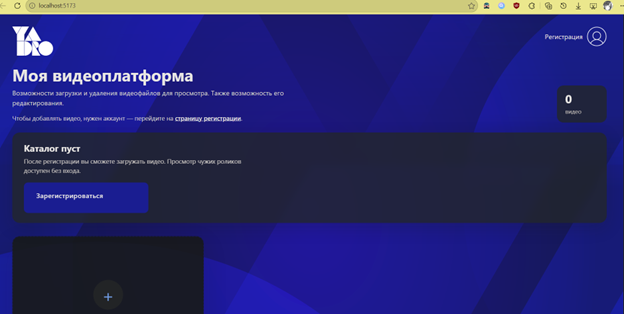
\includegraphics[width=0.92\textwidth]{img/Screenshot_1.png}
  \caption{Главная страница — каталог видео для незарегистрированного пользователя}
  \label{fig:catalog-guest}
\end{figure}

Страница регистрации показана на рисунке~\ref{fig:register}. Она включает форму ввода данных пользователя и возможность получения кода доступа.

\begin{figure}[H]
  \centering
  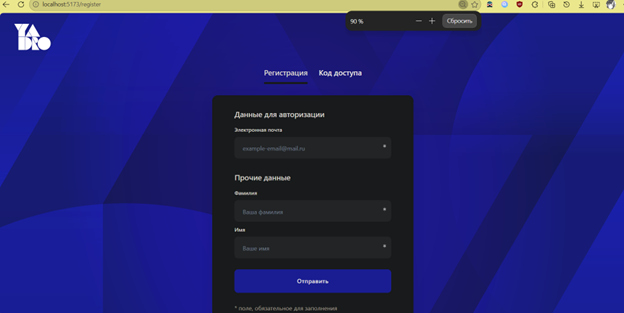
\includegraphics[width=0.92\textwidth]{img/Screenshot_2.png}
  \caption{Страница регистрации пользователя}
  \label{fig:register}
\end{figure}

После добавления видео в систему каталог заполняется карточками, содержащими информацию о роликах и действия для работы с ними (рисунок~\ref{fig:catalog-full}).

\begin{figure}[H]
  \centering
  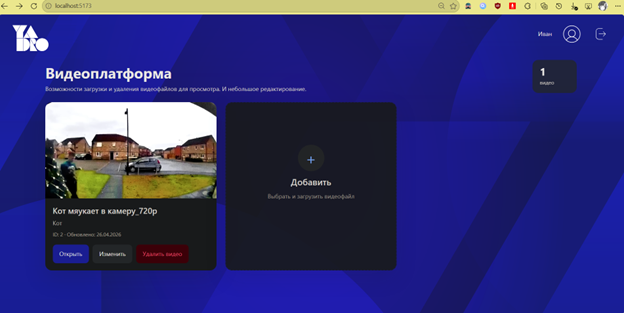
\includegraphics[width=0.92\textwidth]{img/Screenshot_3.png}
  \caption{Каталог с загруженными видео}
  \label{fig:catalog-full}
\end{figure}

На странице просмотра видео (рисунок~\ref{fig:view}) отображается сам видеоплеер и блок комментариев, позволяющий взаимодействовать с контентом.

\begin{figure}[H]
  \centering
  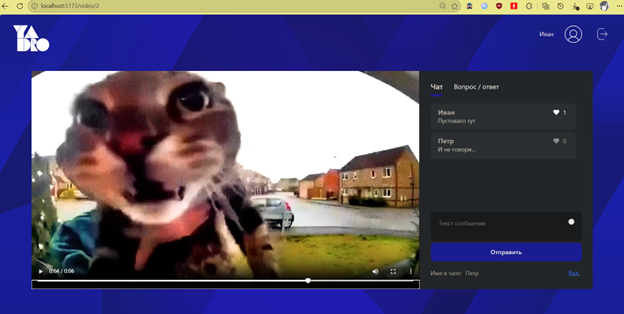
\includegraphics[width=0.92\textwidth]{img/Screenshot_4.png}
  \caption{Страница просмотра видео с комментариями}
  \label{fig:view}
\end{figure}

\chapter{Выводы}

В ходе выполнения расчётно-графической работы была разработана тестовая видеоплатформа, реализующая взаимодействие клиентской и серверной частей. Пользователь имеет возможность зарегистрироваться, просматривать каталог видео, загружать новые файлы, редактировать информацию о них и переходить к странице просмотра с комментариями.

В процессе работы были применены современные технологии веб-разработки: FastAPI для серверной части, React для клиентской части, а также PostgreSQL для хранения данных. Реализовано взаимодействие между компонентами системы через REST API.

Дополнительно были получены практические навыки настройки окружения, работы с Docker, а также устранения типичных проблем, возникающих при разработке веб-приложений, таких как настройка CORS, согласование адресов между фронтендом и бэкендом и организация работы с файловой системой.

В результате выполненной работы удалось закрепить знания по созданию полноценных веб-приложений и понять основные этапы их разработки — от проектирования структуры до реализации и тестирования.

В качестве дальнейшего развития проекта можно рассмотреть внедрение механизма аутентификации на основе JWT, расширение функционала пользовательского взаимодействия, а также добавление автоматизированного тестирования.